% Format A0, orientation paysage (landscape), taille de police de base 25pt
%\documentclass[20pt, a0paper, landscape]{tikzposter}
\documentclass[20pt, a0paper, landscape, margin=1.5cm, colspace=1.5cm, blockverticalspace=1.5cm]{tikzposter}
\tikzposterlatexaffectionproofoff % Enlève le petit texte "Tikzposter" en bas à droite
%\geometry{paperwidth=118.9cm, paperheight=84.1cm, margin=2cm} % Réduit les marges extérieures
%\geometry{a0paper, landscape, margin=2cm}
% ==============================================================================
% PACKAGES
% ==============================================================================
\usepackage[english]{babel} % Pour avoir l'anglais
\usepackage[utf8]{inputenc}
\usepackage[T1]{fontenc}
\usepackage{amsmath, amssymb}
\usepackage{graphicx}
\usepackage{lipsum} % Pour générer du faux texte (à retirer plus tard)
\usepackage{tabularx}
\usepackage{booktabs}
\usepackage{biblatex}
\usepackage{csquotes}
\usepackage{caption}
\usepackage{wrapfig}
\addbibresource{biblio.bib}

\renewcommand*{\bibfont}{\small} % ou \footnotesize si tu as vraiment beaucoup de sources

% ==============================================================================
% THEME ET COULEURS (C'est ici que tu rends le poster "joli")
% ==============================================================================
% Tikzposter propose plusieurs thèmes de base: 
% Default, Rays, Basic, Simple, Envelope, Wave, Board, Autumn, Desert
\usetheme{Default}

% Tu peux aussi changer la palette de couleurs indépendamment du thème:
% Default, Australia, Britain, Sweden, Spain, Russia, Denmark, Germany
\usecolorstyle{Default}

% Pour personnaliser la couleur globale du fond si le thème ne te plaît pas
% \colorlet{backgroundcolor}{blue!10!white}

% ==============================================================================
% EN-TÊTE (TITRE, AUTEURS, LOGOS)
% ==============================================================================
\title{Cross-disciplinary applications of 
the Toulbar2 solver}

\author{
    Hugo Garcia, Philippe Gauthier, Marco Sanfilippo, Mathis Francine-Habas
}

\institute{University of Toulouse \& IRIT Laboratory}

%\titlegraphic{
%    \begin{tabular}{@{}c@{\hspace{15cm}}c@{}}
%        
\includegraphics[height=5cm]{./images/logo_UT.png} & 
%        
\includegraphics[height=5cm]{./images/logo_irit.png}
%    \end{tabular}
%}

% ==============================================================================
% DÉBUT DU POSTER
% ==============================================================================
\begin{document}

\maketitle

\begin{columns}

    % --------------------------------------------------------------------------
    % COLONNE 1 (Gauche): Intro & Contexte
    % --------------------------------------------------------------------------
    \column{0.33} % Prend 33% de la largeur
    
    \block{Abstractz}{
        The valued constraint satisfaction problem (VCSP) or weighted constraint
satisfaction problem (WCSP) is  a generalization of the classic CSP. We try to find 
an assignment of minimal cost to a
set of variables given soft and hard constraints. It is usually solved using a branch-and-bound
search (BnB). 

By finding a good lower bound to a given instance, subtrees of the BnB can
be quickly pruned to efficiently find an optimal solution. This paper studies the cross-disciplinary
application of the solver Toulbar2, ranging from solving difficult combinatorial problems,
to real-world application such as bioinformatics and resource management and finally
artificial intelligence. In many cases where the problem was able to be written using the
VCSP framework, Toulbar2 was able to outperform other state-of-the-art solvers.
        
    }
    
    \block{Combinatorial problem solving}{
        \textbf{Cluster editing for graphs}

        Zahn’s decision problem can be described as the cluster editing problem. Given a graph,
        what is the minimal number of operations (adding edges, removing edges) needed to create
        a disjoint union of cliques. Below an exemple of the cluster editing problem:
        \begin{tikzfigure}[Example of SMC: Robust Supply Chain with Different Network Size.]
        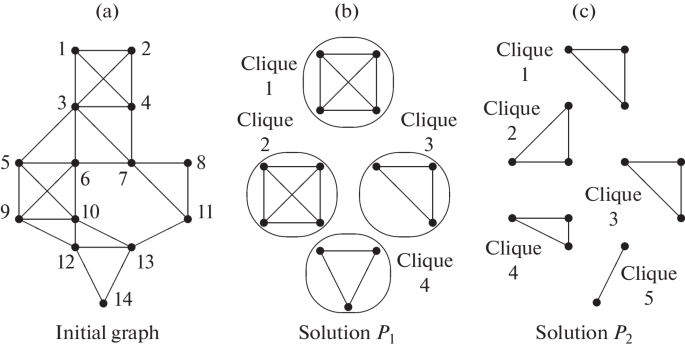
\includegraphics[width=0.7\linewidth]{./images/cluster_editing.png}
        \end{tikzfigure}
        By transforming the cluster editing problem into a VCSP and solving it using Toulbar2, Mhamdi and Naanaa (2014) obtained results much better than the fixed
        parameter algorithm for both sparse and dense graphs.
        \newline

        \textbf{A complicated chess problem}

        \begin{wrapfigure}{l}{0.3\linewidth} % {l} for left, 35% of width
            \centering
            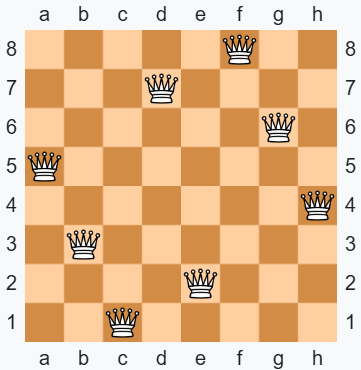
\includegraphics[width=\linewidth]{images/nqueens.png}
            \captionof{figure}{8-Queens example} % Optional caption
        \end{wrapfigure}

        The $N$-Queen problem is a non-trivial mathematical problem that looks for a placement of $N$ queens on a chessboard of size $N$ by $N$ where no two queens are threatening each other. The figure to the left shows an example of a solution where $n = 8$.
        The weighted $N$-Queen problem is the difficult optimization problem of minimizing the cost of the $N$-Queen if every tile incurs a cost. By modeling the weighted $N$-Queen problem as a VCSP, Sewa et al. (2022) demonstrated that Toulbar2 significantly outperforms other state-of-the-art solvers.
        \newline
        \newline
        \newline

        Other problems such as the quadratic assignement problem, the knapsack problem with conflict graph and discrete integrations were also solved using the VCSP framework and showed
        good performance of the Toulbar2 solver.
        }

    % --------------------------------------------------------------------------
    % COLONNE 2 (Milieu): L'État de l'art (Le cœur)
    % --------------------------------------------------------------------------
    \column{0.34} % Légèrement plus large pour le cœur du sujet
    
    % Tu peux forcer une couleur spécifique pour UN bloc important
    \colorlet{blocktitlebgcolor}{blue!80!black} % Change la couleur du titre du bloc
    \block{Bioinformatics \& Life Sciences}{

        \textbf{Computational Protein Design (CPD)}

        CPD aims to create artificial proteins by identifying the amino acid sequence that minimizes the protein's energy, known as the Global Minimum Energy Conformation (GMEC). This is an NP-hard optimization problem due to the vast search space created by the numerous possible side-chain conformations, called rotamers.

        \textbf{Modeling with CFNs and Toulbar2}

        To solve this, the protein structure is mapped into a Cost Function Network (CFN): residues become variables, rotamers become values, and physical interactions are encoded as costs. Toulbar2 uses advanced branch-and-bound and pruning techniques not only to find the exact GMEC, but also to enumerate near-optimal solutions to analyze the complex fitness landscape of the protein.

        \vspace{0.5cm}
        \begin{tikzfigure}[BMC-H homohexamer of bacterial microcompartment (BMC) shell.]
        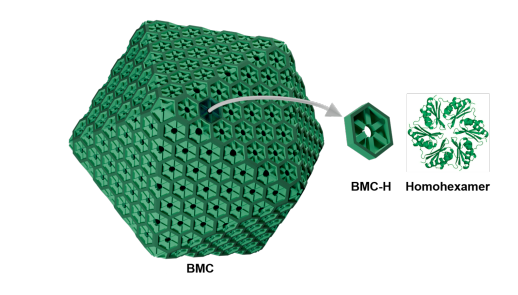
\includegraphics[width=0.7\linewidth]{./images/schema_bmc_partie3.png} 
        \end{tikzfigure}
        \vspace{0.5cm}

        \textbf{Hybrid Deep Learning Approaches}

        Recently, hybrid approaches have emerged to tackle multi-state design. By combining deep learning models (which produce scoring functions) with Toulbar2's exact optimization under explicit constraints, researchers can successfully design complex, symmetrical multi-component proteins—like the homohexamer shown above—while simultaneously avoiding undesirable negative states.
    }
    
    % Remettre la couleur par défaut pour les blocs suivants
    \colorlet{blocktitlebgcolor}{black!80} 
    \block{Recherche Opérationnelle \& Planification}{
        Le formalisme $WCSP$ performe dans la modélisation d'environnements complexes en combinant des règles strictes (contraintes dures) 
        et l'optimisation de critères de qualité (contraintes souples).
        
        \vspace{1cm}
        \begin{center}
        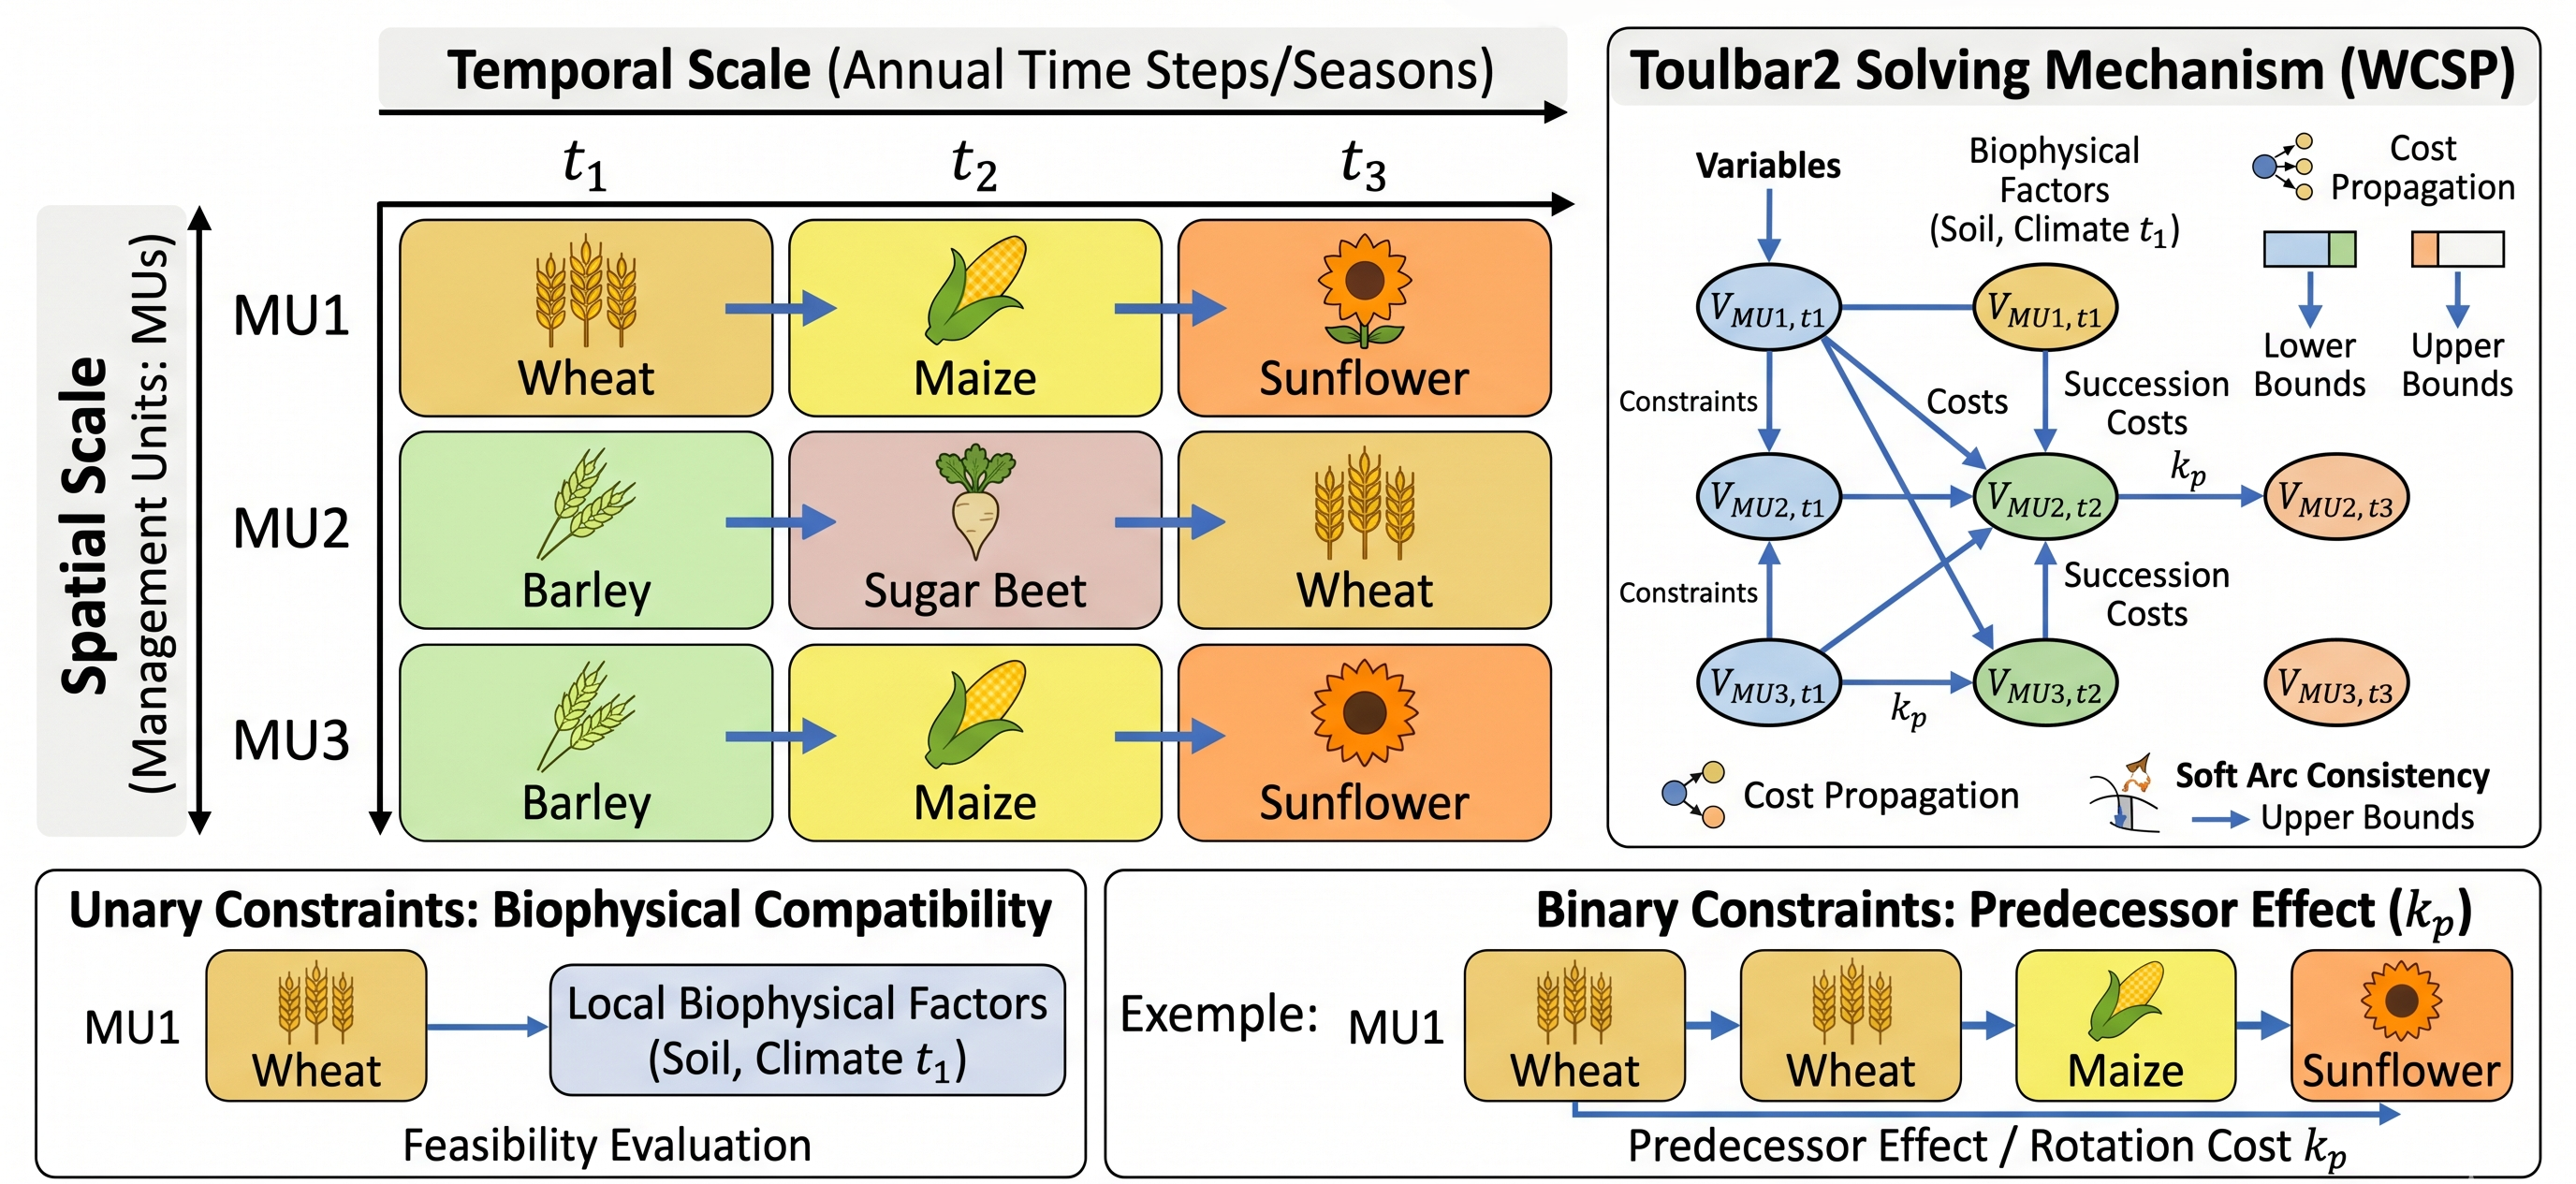
\includegraphics[width=\linewidth]{./images/crop_alloc.png}
        
        
        \end{center}
    }

    % --------------------------------------------------------------------------
    % COLONNE 3 (Droite): Limites, Futures pistes & Biblio
    % --------------------------------------------------------------------------
    \column{0.33}
    
    \block{Artificial Intelligence \& Machine Learning}{
        Toulbar2 struggles with real world applications since 
        exhaustive search creates computational bottlenecks on large instances. 
        We can integrate machine learning, introducing new ways to improve the 
        solution quality. For example, algorithms like KOCO SMC 
        handle large instances by tracking probability bounds during the inference process. 
        This early evaluation prevents the solver from performing exhaustive enumerations.

        \begin{tikzfigure}[Example of SMC: Robust Supply Chain with Different Network Size.[cite: 1072]]
        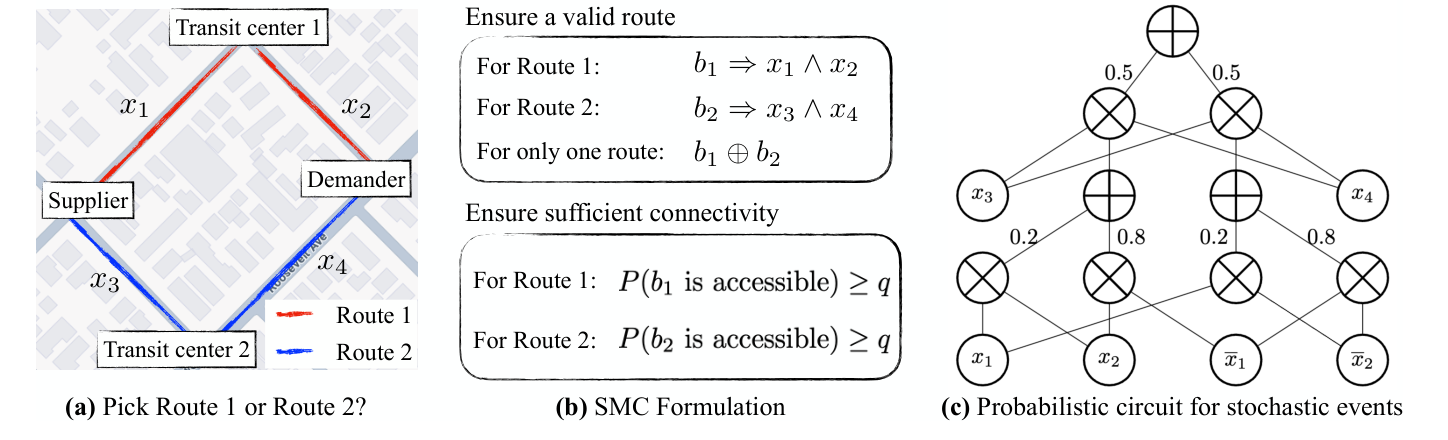
\includegraphics[width=\linewidth]{images/smc_example.png}
        \end{tikzfigure}

        Deep learning models can also transform raw sensory data directly 
        into Graphical Models. This integration merges the perception of neural networks 
        with the exact reasoning of constraint solvers to increase overall flexibility.
        For example, a neural network can translate unmapped protein 
        structures or raw images into cost matrices, allowing Toulbar2 to 
        focus exclusively on executing the exact discrete optimization.
    }
    
    \block{Conclusion}{
The was to understand how a solver based on CFNs, such
as Toulbar2, established itself across such diverse disciplines. 
The answer lies in combining the expressiveness 
of the WCSP formalism with the power of its local consistency algorithms 
(EDAC,VAC, OSAC).

This  demonstrates that Toulbar2 has continuously evolved to adapt to different 
problems. It first became essential in bioinformatics for processing
dense molecular networks. Then proved its competitiveness in resource 
planning by integrating sophisticated global constraints.

We've also seen that to what extent can constraint solvers like Toulbar2 be 
integrated into the training of deep learning model
to correct their logical errors. In the longer term, we may witness the 
emergence of a standardized hybrid AI.
    }

    {
        \colorlet{blocktitlebgcolor}{black!80}       % Fond du titre (gris très foncé)
        \colorlet{blocktitlefgcolor}{white}          % Texte du titre (blanc)
        \colorlet{blockbodybgcolor}{yellow!10!white} % Fond du bloc (jaune très pâle)

        \block{References}{
            \vspace{-1cm}            
            \printbibliography[heading=none] 
        }
            Li, J., Jiang, N., Xue, Y. (2025). 
    Solving Satisfiability Modulo Counting Exactly with 
    Probabilistic Circuits. arXiv:2503.01009. [cite: 1072]
    }
\end{columns}

\end{document}